\hypertarget{sec:intro}{%
\section{Introduction}\label{sec:intro}}

Network slicing places services with very different tolerances on shared
user-plane resources. A URLLC slice tolerates a few milliseconds of
queueing; an eMBB slice is judged on sustained throughput; an mMTC slice
on delivery of sparse reports. When an intrusion detector flags a user
equipment (UE), the operator can rate-limit or block its traffic at the
user-plane function (UPF). Neither action is free. A benign UE that is
wrongly blocked loses its service, and a rate-limited bursty URLLC
client misses its deadline. The cost of a false alarm is therefore set
by the \emph{action} taken and by the \emph{slice} in which it is taken,
not by the alarm alone \cite{sommer2010outside, arp2022dos}.

Recent work has made the false-alarm side of intrusion detection
statistically controllable. Conformal outlier tests give finite-sample
false-positive or false-discovery guarantees \cite{bates2023outliers}.
Several 2025--2026 detectors calibrate alert thresholds against an
explicit false-positive budget using conformal risk control or conformal
evaluation
\cite{youssef2026caliburn, barrett2026firce, farzaneh2025ccoad, barbero2022transcendent}.
What these methods certify is an \emph{alert-level} quantity.
Intrusion-response work, conversely, optimises the choice of defensive
actions, but with model-based guarantees that hold only relative to an
assumed attacker and system model
\cite{hammar2022optimalstopping, hammar2024dynamic, zonouz2014rre}.
Neither line of work certifies the quantity an operator of a sliced
network is accountable for: the fraction of benign users in each slice
whose service-level agreement (SLA) is broken \emph{because of} the
mitigation.

This paper asks one question:

\begin{quote}
\emph{In a sliced 5G user plane where detector-triggered mitigation is
calibrated offline, does certifying each slice's action-induced
SLA-violation risk directly admit more attack mitigation than certifying
each slice's false-positive rate, at the same per-slice budgets and
confidence level, and under what conditions?}
\end{quote}

The question is not rhetorical. We show (Lemma 1) that when the
user-plane scheduler is \emph{monotone} (removing traffic never worsens
the service of other UEs), the action-induced collateral of a slice is
bounded by its acted-benign fraction. A per-slice false-positive-rate
certificate is then also a valid collateral certificate. Direct
certification can only win through the gap between the two, which we
call the \emph{harm ratio}, and must pay for it with a larger hypothesis
space and the need to evaluate counterfactual outcomes.

\textbf{Contributions.}

\begin{enumerate}
\def\labelenumi{\arabic{enumi}.}
\tightlist
\item
  We formalise \emph{action-induced collateral risk} per slice against
  the no-action counterfactual, and prove that under scheduler
  monotonicity it is upper-bounded by the per-slice acted-benign
  fraction (Lemma 1). This identifies per-slice certified false-positive
  control as the correct strong baseline and isolates the harm ratio as
  the only source of possible gain (Remark 1).
\item
  We give a replay-based certification procedure, RC-SIR, that applies
  Learn-then-Test (LTT) risk control \cite{angelopoulos2025ltt} over a
  space of 1331 per-slice multi-action policies. It uses union-null
  p-values across slices and either Bonferroni or data-split
  fixed-sequence family-wise error control. We also prove a transfer
  result for calibrating on a replay twin with bounded error
  (Proposition 2). The statistical machinery is existing; the
  contribution is the formulation, the structural result that determines
  when the machinery helps, and its measured consequences.
\item
  We report a reproducible simulation study of a three-slice user plane
  with a detector deployed under domain shift (Isolation Forest, pool
  AUC 0.892). Over 200 calibration/test splits:

  \begin{itemize}
  \tightlist
  \item
    No certified method exceeded its budgets.
  \item
    Uncalibrated constrained selection did, in 25.5\% of splits at 100
    calibration episodes.
  \item
    With fixed-sequence testing, direct certification delivered 0.417 of
    attack traffic, against 0.458 for per-slice FPR certification
    (better in 93.5\% of paired splits).
  \item
    The advantage disappears with small calibration sets, at halved or
    doubled budgets, and with Bonferroni control. Multi-action policies
    brought no measurable benefit.
  \end{itemize}
\end{enumerate}

All results come from a fluid simulator, not from a 5G testbed.
Section\textasciitilde{}\ref{sec:limits} discusses what this does and
does not establish.

\hypertarget{sec:related}{%
\section{Related Work}\label{sec:related}}

\textbf{Evaluation validity of ML-based intrusion detection.}

\begin{itemize}
\tightlist
\item
  Operational cost of errors and evaluation pitfalls are long-standing
  concerns \cite{sommer2010outside, arp2022dos}.
\item
  Benchmark datasets contain labelling and design flaws
  \cite{engelen2021troubleshooting, flood2024smells}.
\item
  Detectors degrade sharply across domains \cite{layeghy2023xcross}.
\item
  5G-specific datasets report near-perfect detection
  \cite{siriwardhana2025nidd, khan2023slicesecure, amponis2022pfcp},
  while adversarial evaluation of 5G-core detectors exposes fragility
  \cite{manca2026sage5gc}.
\end{itemize}

Our first simulator version reproduced the near-perfect-detection
artefact; we discarded it for that reason
(Section\textasciitilde{}\ref{sec:limits}).

\textbf{Calibrated intrusion detection.} Conformal p-values support
exact FDR control for outlier detection \cite{bates2023outliers}.
TRANSCENDENT uses conformal evaluation to reject drifting samples
\cite{barbero2022transcendent}. FIRCE couples conformal evaluators with
drift-triggered retraining \cite{barrett2026firce}. CALIBURN sets
streaming alert thresholds by regime-dependent conformal risk control
under a false-positive budget \cite{youssef2026caliburn}. An online
conformal detector controls a smoothed false-discovery rate
\cite{farzaneh2025ccoad}. All of these certify detector outputs. None
certifies the service-level effect of the action taken on an alert, and
none partitions the guarantee by slice. Our per-slice FPR baseline is
the natural slice-stratified extension of these methods.

\textbf{Risk control.}

\begin{itemize}
\tightlist
\item
  Conformal risk control bounds monotone losses
  \cite{angelopoulos2024crc}.
\item
  LTT handles non-monotone and multiple risks by multiple testing
  \cite{angelopoulos2025ltt}.
\item
  Weighted and online variants address shift
  \cite{tibshirani2019weighted, barber2023beyond, gibbs2021aci}.
\item
  Conformal policy control regulates a new policy against a safe
  reference policy \cite{prinster2026cpc}.
\item
  Prediction-powered risk control uses unlabelled data to reduce
  conservativeness \cite{einbinder2025ssrc}.
\end{itemize}

RC-SIR uses LTT without modification. Its departure is in what is
certified (counterfactual, slice-indexed SLA outcomes) and in the
structural analysis of when certification of that quantity is worth its
cost.

\textbf{Intrusion response and mitigation.}

\begin{itemize}
\tightlist
\item
  Hammar and Stadler derive threshold-structured optimal response
  policies via optimal stopping and stochastic games
  \cite{hammar2022optimalstopping, hammar2024dynamic}.
\item
  RRE selects responses in a partially observable game
  \cite{zonouz2014rre}.
\item
  Switch-native systems mitigate volumetric DDoS at line rate
  \cite{liu2021jaqen}.
\end{itemize}

These works optimise response quality under a model; they do not provide
distribution-free bounds on collateral harm. Our policies have the
threshold structure these works motivate.

\textbf{Slicing.}

\begin{itemize}
\tightlist
\item
  RAN slicing with performance isolation \cite{foukas2017orion}.
\item
  Overbooking \cite{salvat2018overbooking} and asymmetric SLA-cost
  forecasting \cite{bega2019deepcog} show that slices share and borrow
  capacity, which is the coupling our scheduler models.
\item
  Network digital twins \cite{ferriolgalmes2023routenetfermi} are
  candidate replay engines for the counterfactual evaluation that RC-SIR
  requires.
\item
  Attacks on learned slicing controllers produce slice-dependent SLA
  violations \cite{tashman2026adversarial}.
\end{itemize}

Table\textasciitilde{}\ref{tab:comparison} summarises the comparison.

\begin{table*}[!t]
\centering
\caption{Comparison with the closest approaches (qualitative columns from the cited papers' abstracts; "Measured here" from our experiments).}
\label{tab:comparison}
\footnotesize
\resizebox{\linewidth}{!}{%
\begin{tabular}{p{0.15\linewidth}p{0.15\linewidth}p{0.15\linewidth}p{0.15\linewidth}p{0.15\linewidth}p{0.15\linewidth}}
\toprule
\textbf{Approach} & \textbf{What it provides} & \textbf{Assumptions / limits} & \textbf{Difference in this work} & \textbf{Measured here} & \textbf{Where it is better} \\
\midrule
Conformal outlier / FPR control \cite{bates2023outliers,youssef2026caliburn} & Finite-sample alert-level FPR/FDR or FP-budget control & Exchangeability; certifies alerts, not action outcomes; not slice-indexed & Certifies slice-indexed SLA outcomes of actions & 1\% FPR operating point: 0.775 attack delivered & Needs no replay; simplest to deploy \\
Per-slice certified FPR (Corollary 1, our baseline) & Collateral certificate via Lemma 1 & Requires monotone scheduler (A3) & Direct certification exploits harm ratio $<$ 1 & 0.458 attack delivered & Small calibration sets, halved/doubled budgets, expensive replay \\
LTT / CRC \cite{angelopoulos2025ltt,angelopoulos2024crc} & Generic risk-control machinery & i.i.d. calibration & Used unchanged; we add the counterfactual slice-collateral formulation and structural analysis & Bonferroni variant: 0.498; fixed-sequence: 0.417 & n/a \\
Optimal-stopping / game-theoretic response \cite{hammar2022optimalstopping,zonouz2014rre} & Optimal threshold response under a model & Attacker/system model; no distribution-free collateral bound & Distribution-free per-slice collateral certificate & Not reproduced (Section 8) & Optimises response timing, which our episodic model does not \\
Conformal policy control \cite{prinster2026cpc} & Risk-controlled deviation from a safe policy & Generic; safe reference policy & Network-specific counterfactual loss, slice structure & Not compared (different setting) & Online policy improvement \\
Pooled certification (ablation) & One certificate across slices & Ignores slice heterogeneity & Per-slice budgets & 0.566 attack delivered & None observed \\
\bottomrule
\end{tabular}
}
\end{table*}

\hypertarget{sec:model}{%
\section{System Model and Problem Formulation}\label{sec:model}}

\textbf{User plane.} An egress link of capacity \(C\) serves slices
\(s \in \mathcal{S}=\{\mathrm{eMBB},\mathrm{URLLC},\mathrm{mMTC}\}\).
Slice \(s\) is guaranteed \(g_s C\) and may borrow idle capacity up to
\(C\), as in hierarchical token-bucket sharing. Each slice has a finite
FIFO buffer; within a slice, drops and queueing delay are shared by its
UEs. Time is slotted.

\textbf{Episodes and detector.} An episode \(e\) consists of an
observation window of \(T_o\) slots and an action window of \(T_a\)
slots. A detector maps the observation-window features of UE \(u\) to a
score \(z_u \in [0,1]\). \(\mathcal{B}_s(e)\) is the set of benign UEs
of slice \(s\) in episode \(e\).

\textbf{Policies.} A policy \(\pi_\lambda\) is parameterised by
\(\lambda=(\tau_s,a_s)_{s\in\mathcal{S}}\), a threshold and an action
\(a_s\in\{\mathsf{RL},\mathsf{B}\}\) (rate-limit to a slice-specific
cap, or block). Every UE of slice \(s\) with \(z_u\ge\tau_s\) receives
action \(a_s\) for the whole action window; \(\tau_s=\infty\) means no
action. \(\pi_0\) takes no action. With five thresholds and two actions
per slice, \(|\Lambda|=11^3=1331\).

\textbf{SLA outcomes.} \(V_u(e;\pi)\in\{0,1\}\) indicates that benign UE
\(u\) violates its slice SLA during the action window under policy
\(\pi\):

\begin{itemize}
\tightlist
\item
  eMBB: delivered/offered ratio below 0.90;
\item
  URLLC: 95th-percentile queueing delay above 2 slots, or delivery below
  0.99;
\item
  mMTC: delivery below 0.95.
\end{itemize}

\textbf{Definition 1 (action-induced collateral).} For slice \(s\) and
policy \(\pi_\lambda\),
\[L^{c}_s(e;\lambda)=\frac{1}{|\mathcal{B}_s(e)|}\sum_{u\in\mathcal{B}_s(e)}\mathbb{1}\{V_u(e;\pi_\lambda)=1,\;V_u(e;\pi_0)=0\},\qquad R^{c}_s(\lambda)=\mathbb{E}_e[L^{c}_s(e;\lambda)].\]
The counterfactual \(\pi_0\) separates harm caused by mitigation from
harm caused by the attack itself.

\textbf{Objective.} Let \(L^{a}(e;\lambda)\in[0,1]\) be the fraction of
attack traffic delivered under \(\pi_\lambda\) in an episode containing
attackers, and \(R^a(\lambda)\) its expectation. The operator seeks
\[\min_{\lambda\in\Lambda} R^{a}(\lambda)\quad\text{s.t.}\quad R^{c}_s(\lambda)\le\alpha_s\;\;\forall s\in\mathcal{S},\]
and requires the selected \(\hat{\lambda}\) to satisfy all constraints
with probability at least \(1-\delta\) over the calibration data.

\textbf{Assumptions.}

\begin{itemize}
\tightlist
\item
  \textbf{A1:} calibration and deployment episodes are i.i.d. draws from
  the same distribution.
\item
  \textbf{A2:} \(L^c_s(e;\lambda)\) can be evaluated for every
  \(\lambda\) on a calibration episode by replaying its traffic, either
  in a replay engine or in a twin whose error is bounded as in
  Proposition 2.
\item
  \textbf{A3 (monotone scheduling):} if the offered traffic of a set of
  UEs is reduced pointwise in time, no other UE's delivered fraction
  decreases and no other UE's queueing delay increases.
\end{itemize}

A3 holds for work-conserving fair schedulers with per-UE policing
applied before queueing. It can fail with congestion-control feedback or
non-work-conserving shapers. For our simulator we verify it numerically
rather than analytically (Section\textasciitilde{}\ref{sec:results}).

\textbf{Lemma 1.} Under A3, for every episode \(e\), policy \(\lambda\)
and slice \(s\),
\[L^{c}_s(e;\lambda)\le F_s(e;\tau_s):=\frac{1}{|\mathcal{B}_s(e)|}\sum_{u\in\mathcal{B}_s(e)}\mathbb{1}\{z_u\ge\tau_s\}.\]

\emph{Proof.} Let \(u\in\mathcal{B}_s(e)\) with \(z_u<\tau_s\), so \(u\)
is not acted on. Under \(\pi_\lambda\) the offered traffic of every
other UE is pointwise no larger than under \(\pi_0\), and \(u\)'s own
traffic is unchanged. By A3, \(u\)'s delivered fraction is no smaller
and its delay no larger under \(\pi_\lambda\). Hence
\(V_u(e;\pi_\lambda)\le V_u(e;\pi_0)\), and \(u\) contributes zero to
\(L^c_s\). Only acted UEs can contribute, each at most
\(1/|\mathcal{B}_s(e)|\). $\square$

\textbf{Remark 1 (where a gain can come from).} Write
\(R^{c}_s(\lambda)=\rho_s(\lambda)\,\Phi_s(\tau_s)\), with
\(\Phi_s(\tau)=\mathbb{E}[F_s(e;\tau)]\) and harm ratio
\(\rho_s\in[0,1]\). A per-slice FPR certificate admits only thresholds
with \(\Phi_s(\tau_s)\le\alpha_s\). Direct certification admits
\(\Phi_s(\tau_s)\le\alpha_s/\rho_s\). Direct certification can therefore
select more aggressive thresholds only when \(\rho_s\) is substantially
below one \emph{and} the threshold grid contains points in the band
\((\alpha_s,\alpha_s/\rho_s]\), after allowing for the statistical
margin of each test. The remark is an identity, but it predicts where
the gain should and should not appear, and we test that prediction.

\hypertarget{sec:method}{%
\section{Certification Procedure}\label{sec:method}}

For each calibration episode \(e_i\), \(i=1,\dots,n\), the replay engine
evaluates \(L^c_s(e_i;\lambda)\) and \(L^a(e_i;\lambda)\) for all
\(\lambda\in\Lambda\). Let \(\hat{R}_s(\lambda)\) be the empirical mean
of \(L^c_s\) over the calibration episodes. For each \(\lambda\) we test
the union null \(H_\lambda:\exists s,\;R^c_s(\lambda)>\alpha_s\) with
the p-value
\[p_\lambda=\max_{s\in\mathcal{S}} p^{\mathrm{HB}}\big(\hat{R}_s(\lambda);\alpha_s,n\big),\]
where \(p^{\mathrm{HB}}\) is the Hoeffding--Bentkus p-value for
\([0,1]\)-bounded losses used in LTT \cite{angelopoulos2025ltt}. The
certified set \(\hat{\Lambda}\) is obtained with family-wise error rate
(FWER) control at level \(\delta\), in one of two variants:

\begin{itemize}
\tightlist
\item
  \textbf{Bonferroni (RC-SIR):}
  \(\hat{\Lambda}=\{\lambda: p_\lambda\le\delta/|\Lambda|\}\).
\item
  \textbf{Fixed sequence (RC-SIR-FS):} the calibration set is split in
  half. The first half orders policies by
  \(\max_s \hat{R}_s(\lambda)/\alpha_s\), ties broken by empirical
  attack delivery. The second half tests \(H_\lambda\) in that order at
  level \(\delta\), stopping at the first non-rejection.
\end{itemize}

The deployed policy is
\(\hat{\lambda}=\arg\min_{\lambda\in\hat{\Lambda}}\hat{R}^a(\lambda)\),
computed on the full calibration set, with \(\pi_0\) as the fallback
when \(\hat{\Lambda}=\emptyset\). Algorithm 1 summarises the procedure.

\begin{algorithm}[!t]
\caption{RC-SIR / RC-SIR-FS certification and selection}\label{alg:rcsir}
\begin{algorithmic}[1]
\REQUIRE calibration episodes $e_1,\dots,e_n$; policy set $\Lambda$; budgets $\alpha_s$; level $\delta$; variant
\FOR{$i=1$ \TO $n$} \STATE replay $e_i$ under every $\lambda\in\Lambda$ and $\pi_0$; record $L^c_s(e_i;\lambda)$, $L^a(e_i;\lambda)$ \ENDFOR
\IF{variant = Bonferroni}
  \STATE $p_\lambda\gets\max_s p^{\mathrm{HB}}(\hat R_s(\lambda);\alpha_s,n)$; \quad $\hat\Lambda\gets\{\lambda:p_\lambda\le\delta/|\Lambda|\}$
\ELSE
  \STATE split calibration set into halves $D_1,D_2$; order $\Lambda$ by $\max_s\hat R^{(D_1)}_s(\lambda)/\alpha_s$
  \STATE $\hat\Lambda\gets\emptyset$; \FOR{$\lambda$ in that order} \IF{$\max_s p^{\mathrm{HB}}(\hat R^{(D_2)}_s(\lambda);\alpha_s,|D_2|)\le\delta$} \STATE $\hat\Lambda\gets\hat\Lambda\cup\{\lambda\}$ \ELSE \STATE \textbf{break} \ENDIF \ENDFOR
\ENDIF
\STATE \textbf{return} $\arg\min_{\lambda\in\hat\Lambda}\hat R^a(\lambda)$ if $\hat\Lambda\neq\emptyset$, else $\pi_0$
\end{algorithmic}
\end{algorithm}

\textbf{Proposition 1 (validity).} Under A1--A2, both variants satisfy
\(\Pr\{\forall s:\ R^c_s(\hat{\lambda})\le\alpha_s\}\ge1-\delta\).

\emph{Proof.}

\begin{enumerate}
\def\labelenumi{\arabic{enumi}.}
\tightlist
\item
  Under \(H_\lambda\) there is a slice \(s^\ast\) with
  \(R^c_{s^\ast}(\lambda)>\alpha_{s^\ast}\). Since
  \(p_\lambda\ge p^{\mathrm{HB}}_{s^\ast}\) and \(p^{\mathrm{HB}}\) is
  super-uniform under that null, \(p_\lambda\) is a valid p-value for
  \(H_\lambda\).
\item
  Bonferroni controls the FWER at \(\delta\). Fixed-sequence testing
  does too, because the ordering is a function of the first half only,
  and the second half is independent of it under A1.
\item
  On the complement of a family-wise error, every
  \(\lambda\in\hat{\Lambda}\) satisfies all constraints, so any
  selection rule over \(\hat{\Lambda}\), including one that uses all
  calibration data, inherits the guarantee.
\item
  The fallback \(\pi_0\) has \(R^c_s=0\). $\square$
\end{enumerate}

The result is a direct consequence of LTT \cite{angelopoulos2025ltt};
we state it to make the union-null construction and the selection step
explicit.

\textbf{Corollary 1 (per-slice FPR baseline).} Certify for each slice
the smallest threshold with \(\Phi_s(\tau_s)\le\alpha_s\), testing
thresholds from the most conservative downwards (valid fixed-sequence
testing because \(F_s\) is monotone in \(\tau\)) at level
\(\delta/|\mathcal{S}|\), and block above it. By Lemma 1 this also
satisfies the collateral constraints with probability at least
\(1-\delta\). It requires no replay, only benign scores.

\textbf{Proposition 2 (calibration on a twin).} Suppose calibration uses
twin losses \(\tilde{L}^c_s\), and on an event \(E\) with
\(\Pr(E)\ge1-\eta\),
\(|\tilde{R}^c_s(\lambda)-R^c_s(\lambda)|\le\varepsilon_s\) for all
\(\lambda,s\). Certifying the twin at budgets \(\alpha_s-\varepsilon_s\)
yields
\(\Pr\{\forall s: R^c_s(\hat{\lambda})\le\alpha_s\}\ge1-\delta-\eta\).

\emph{Proof.} On \(E\) intersected with the twin certification event,
\(R^c_s(\hat{\lambda})\le\tilde{R}^c_s(\hat{\lambda})+\varepsilon_s\le\alpha_s\).
A union bound completes the proof. $\square$

To estimate \(\varepsilon_s\) we use \(m\) paired twin/real episodes:
\(\hat{\varepsilon}_s=\max_\lambda m^{-1}\sum_j|\tilde{L}^c_s-L^c_s|+\sqrt{\log(3|\Lambda|/\eta)/(2m)}\).
This is valid by Hoeffding's inequality with a union bound, because
\(|\tilde{R}-R|\le\mathbb{E}|\tilde{L}-L|\).

\textbf{Complexity.} Calibration costs \(O(n|\Lambda||\mathcal{S}|)\)
operations for the risk means plus \(O(|\Lambda|)\) p-values. The
dominant cost is replay: \(|\Lambda|\) policy evaluations per
calibration episode, each \(O(UT_a)\) for \(U\) UEs.

\hypertarget{sec:setup}{%
\section{Experimental Setup}\label{sec:setup}}

\textbf{Simulator.}

\begin{itemize}
\tightlist
\item
  Capacity \(C=100\) units/slot, guaranteed shares \((0.55,0.25,0.20)\),
  buffers \((200,12,60)\) units.
\item
  14, 10 and 16 benign UEs per slice; \(T_o=30\), \(T_a=120\) slots.
\item
  With probability 0.6, an episode contains 1--4 attackers, placed in
  eMBB, URLLC and mMTC with probabilities \((0.45,0.15,0.40)\).
\item
  Attack types: constant floods, pulsing floods, and (in deployment
  only) low-and-slow sources.
\item
  Rate-limit caps are \((3.0,1.0,0.5)\) units/slot.
\end{itemize}

All parameters are listed in \texttt{code/sim.py} and recorded in
\texttt{results/results.json}.

\textbf{Training versus deployment regime.} The detector is trained on a
\emph{benchmark} regime. Deployment episodes come from an
\emph{operational} regime that adds:

\begin{itemize}
\tightlist
\item
  more variable heavy eMBB users,
\item
  URLLC alarm bursts and mMTC firmware-update bursts,
\item
  attackers that mimic their slice's packet size in 70\% of cases,
\item
  an unseen low-and-slow attack class.
\end{itemize}

This models the cross-domain degradation documented for real detectors
\cite{layeghy2023xcross}.

\textbf{Detectors.} The primary detector is an Isolation Forest
\cite{liu2008iforest} trained on benign benchmark-regime UEs. Its score
is the empirical quantile of benign training scores, so thresholds are
\(\{0.9,0.95,0.99,0.995,0.999\}\). A gradient-boosting classifier
trained on labelled benchmark-regime UEs is a secondary check. Both use
scikit-learn \cite{pedregosa2011sklearn}. Each detector has seven
per-UE features computed on the observation window only (mean, standard
deviation, maximum, activity fraction, peak-to-mean ratio, mean absolute
increment, mean packet size) plus slice indicators. Deployment pool AUCs
were 0.892 (Isolation Forest) and 0.826 (gradient boosting).

\textbf{Data.} Seeds derive from one master seed (20261102) through
independent \texttt{SeedSequence} streams:

\begin{itemize}
\tightlist
\item
  600 training episodes (benchmark regime);
\item
  a pool of 1500 deployment episodes (62.6\% containing attacks);
\item
  400 high-load deployment episodes (load factor in \([1.1,1.35]\)
  instead of \([0.6,1.1]\)).
\end{itemize}

Every pool episode is replayed under all 1331 policies, \(\pi_0\) and
the oracle (which blocks exactly the attackers), for both detectors and
for a twin that overestimates capacity by 8\%.

\textbf{Protocol.}

\begin{itemize}
\tightlist
\item
  Budgets \(\alpha=(0.05,0.02,0.05)\), \(\delta=0.1\).
\item
  Selection objective: mean delivered attack fraction over calibration
  episodes that contain attackers, plus \(10^{-3}J\) as a tie-breaker,
  where \(J=\sum_s w_s\,\overline{V}_s\) is the weighted benign
  SLA-violation rate with \(w=(0.3,0.5,0.2)\).
\item
  200 random splits of the pool into \(n=500\) calibration and 1000 test
  episodes.
\item
  These settings and the objective were fixed before results were
  computed (Section\textasciitilde{}\ref{sec:limits} records one
  implementation deviation and its correction).
\item
  A split counts as a \emph{violation} if any slice's realised test
  collateral exceeds its budget. Certified methods should violate in at
  most a fraction \(\delta\) of splits.
\end{itemize}

\textbf{Baselines.} All baselines select among the same 1331 policies
and the same replayed outcomes:

\begin{itemize}
\tightlist
\item
  \textbf{Slice-FPR:} Corollary 1, the strongest alert-level competitor.
\item
  \textbf{Pooled LTT:} one shared \((\tau,a)\) certified on
  benign-averaged collateral.
\item
  \textbf{Conformal FPR 1\%:} a single threshold with conformal benign
  FPR at most 1\%, then block. This is the operating point of
  alert-level calibrated detectors.
\item
  \textbf{Fixed threshold:} block above the 99th benign-training
  percentile.
\item
  \textbf{ERM:} minimise empirical \(\hat{R}^a\) subject to
  \(\hat{R}_s\le\alpha_s\), without a statistical margin.
\item
  \textbf{No action and Oracle:} reference points.
\end{itemize}

A model-based optimal-stopping response
\cite{hammar2022optimalstopping} is not reproduced;
Section\textasciitilde{}\ref{sec:limits} explains why.

\hypertarget{sec:results}{%
\section{Results}\label{sec:results}}

\textbf{Assumption checks.}

\begin{itemize}
\tightlist
\item
  \textbf{A3.} Over all \(1500\times1331\times3\) episode--policy--slice
  combinations, collateral never exceeded the acted-benign fraction by
  more than 2.6e-08, which is float32 rounding.
\item
  \textbf{Unit tests.} A randomised test over 1000 arbitrary per-UE
  action patterns found no non-acted UE whose SLA status worsened.
\item
  \textbf{Harm ratio.} Pooled over acted policies it was 0.72, but it
  varies strongly with slice and action
  (Table\textasciitilde{}\ref{tab:harm_ratio}):

  \begin{itemize}
  \tightlist
  \item
    about 0.54 for eMBB at threshold 0.99;
  \item
    about 0.95 for URLLC;
  \item
    0.11 for rate-limiting in mMTC, against 0.99 for blocking there.
  \end{itemize}

  By Remark 1, direct certification can gain mainly in eMBB.
\end{itemize}

\textbf{Validity and the main comparison.}
Table\textasciitilde{}\ref{tab:main} reports the main comparison. No
certified method exceeded its budgets in any of the 200 splits. ERM,
which enforces the budgets only empirically, violated them in 10.0\% of
splits at \(n=500\). As \(n\) decreases this rises to 15.5\% at
\(n=250\) and 25.5\% at \(n=100\) (Fig.\textasciitilde{}\ref{fig:ncal}).
At \(n=500\) the ERM violation frequency equals the nominal \(\delta\),
so at that calibration size the empirical rule is not worse than the
target level; the certificate matters at smaller \(n\). The realised
collateral of the certified methods stayed well below the budgets (for
example 0.018 against 0.05 in eMBB), which shows that the certificates
are conservative. Fig.\textasciitilde{}\ref{fig:collateral} shows the
distribution of realised collateral.

\begin{table*}[!t]
\centering
\caption{Main comparison, Isolation-Forest detector, 200 random splits (n\_cal = 500, n\_test = 1000). Budgets alpha = (0.05, 0.02, 0.05), delta = 0.1. Collateral = mean realised test collateral risk; viol. freq. = fraction of splits where any slice exceeds its budget (target $<$= delta for certified methods).}
\label{tab:main}
\footnotesize
\resizebox{\linewidth}{!}{%
\begin{tabular}{p{0.11\linewidth}rrrrrrr}
\toprule
\textbf{Method} & \textbf{Viol. freq. ($\pm$MC s.e.)} & \textbf{Collateral eMBB} & \textbf{Collateral URLLC} & \textbf{Collateral mMTC} & \textbf{Benign viol. J} & \textbf{Attack delivered} & \textbf{Fallback} \\
\midrule
RC-SIR (ours) & 0.000 $\pm$ 0.000 & 0.0061 & 0.0000 & 0.0032 & 0.0305 & 0.498 & 0.00 \\
RC-SIR-FS (ours) & 0.000 $\pm$ 0.000 & 0.0181 & 0.0024 & 0.0031 & 0.0240 & 0.417 & 0.00 \\
Slice-FPR certified + block & 0.000 $\pm$ 0.000 & 0.0061 & 0.0025 & 0.0031 & 0.0288 & 0.458 & 0.00 \\
ERM (no margin) & 0.100 $\pm$ 0.021 & 0.0191 & 0.0025 & 0.0083 & 0.0243 & 0.409 & 0.00 \\
Pooled LTT & 0.000 $\pm$ 0.000 & 0.0191 & 0.0025 & 0.0000 & 0.0260 & 0.566 & 0.00 \\
Conformal FPR 1\% + block & 0.000 $\pm$ 0.000 & 0.0061 & 0.0000 & 0.0000 & 0.0426 & 0.775 & 0.00 \\
Fixed threshold + block & 0.000 $\pm$ 0.000 & 0.0191 & 0.0025 & 0.0000 & 0.0260 & 0.566 & 0.00 \\
No action & 0.000 $\pm$ 0.000 & 0.0000 & 0.0000 & 0.0000 & 0.0799 & 0.963 & 1.00 \\
Oracle & 0.000 $\pm$ 0.000 & 0.0000 & 0.0000 & 0.0000 & 0.0217 & 0.000 & 0.00 \\
\bottomrule
\end{tabular}
}
\end{table*}

\begin{figure*}[!t]\centering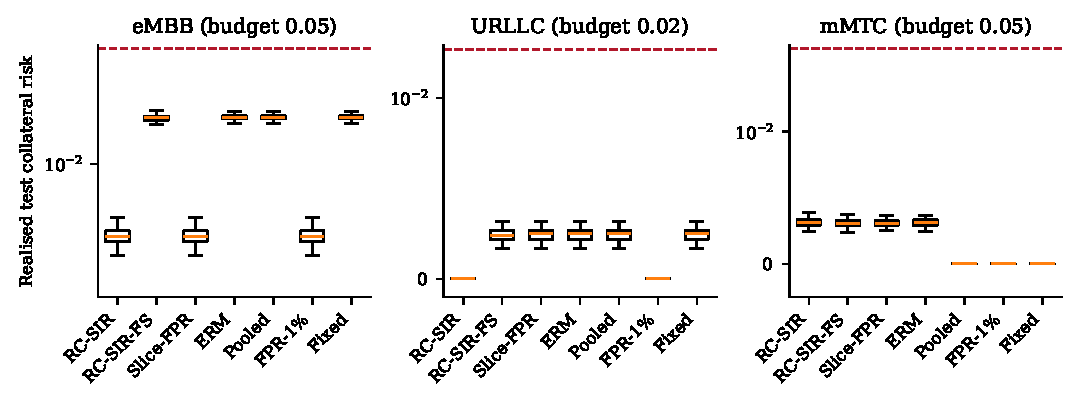
\includegraphics[width=0.95\textwidth]{figures/fig_collateral.pdf}\caption{Realised test collateral per slice over 200 splits (log-linear axis); dashed lines are the budgets.}\label{fig:collateral}\end{figure*}

\textbf{Direct versus FPR certification.} With fixed-sequence testing,
RC-SIR-FS delivered 0.417 of attack traffic, against 0.458 for
Slice-FPR. Paired over identical splits
(Table\textasciitilde{}\ref{tab:paired}), the mean difference was
-0.043, and RC-SIR-FS was better in 93.5\% of splits. The 97.5\%
quantile of the difference was +0.041: in a minority of splits the
half-sample split costs more than the harm-ratio gain.

The modal RC-SIR-FS policy blocked at threshold 0.99 in eMBB, where
Slice-FPR certified only 0.995. At 0.99 the eMBB acted-benign fraction
is 0.035. That is below the 0.05 budget, but too close to it for the
Hoeffding--Bentkus test to certify at level \(\delta/3\) with 500
episodes. The collateral at the same threshold, 0.019, leaves enough
margin. The gain is thus the statistical-margin component of Remark 1,
not the deterministic band.

With Bonferroni control, RC-SIR was \emph{worse} than Slice-FPR in every
split (mean difference +0.040). Correcting over 1331 hypotheses costs
more margin than the harm ratio returns.

Against pooled certification and the alert-level operating points,
direct certification delivered less attack traffic (0.566 for Pooled
LTT, 0.775 for 1\% conformal FPR).

\begin{table*}[!t]
\centering
\caption{Paired comparisons on identical calibration/test splits (200 splits, n\_cal = 500). Negative differences favour A.}
\label{tab:paired}
\footnotesize
\resizebox{\linewidth}{!}{%
\begin{tabular}{lrp{0.15\linewidth}rrr}
\toprule
\textbf{Comparison (A vs B)} & \textbf{Mean diff. attack delivered (A-B)} & \textbf{2.5\% / 50\% / 97.5\% quantile over splits} & \textbf{A better} & \textbf{Tie} & \textbf{Mean diff. J} \\
\midrule
RC-SIR vs Slice-FPR & +0.0402 & +0.0329 / +0.0401 / +0.0476 & 0.000 & 0.000 & +0.0017 \\
RC-SIR vs Pooled LTT & -0.0674 & -0.0853 / -0.0673 / -0.0503 & 1.000 & 0.000 & +0.0045 \\
RC-SIR-FS vs RC-SIR & -0.0828 & -0.0983 / -0.0876 / +0.0000 & 0.965 & 0.015 & -0.0066 \\
RC-SIR-FS vs Slice-FPR & -0.0427 & -0.0554 / -0.0479 / +0.0405 & 0.935 & 0.030 & -0.0048 \\
RC-SIR-FS vs Pooled LTT & -0.1493 & -0.1676 / -0.1541 / -0.0666 & 1.000 & 0.000 & -0.0021 \\
RC-SIR-FS vs ERM & +0.0065 & +0.0000 / +0.0000 / +0.0873 & 0.000 & 0.875 & +0.0000 \\
\bottomrule
\end{tabular}
}
\end{table*}

\textbf{When the advantage disappears.}

\begin{itemize}
\tightlist
\item
  \textbf{Small calibration sets.} At \(n\le250\) RC-SIR-FS often fell
  back to no action, or certified less than Slice-FPR, which needs no
  replay and tests only five monotone thresholds per slice
  (Fig.\textasciitilde{}\ref{fig:ncal}). At \(n=250\) the delivered
  attack fractions were 0.539 versus 0.490; at \(n=1000\), 0.413 versus
  0.453.
\item
  \textbf{Other budgets.} Halving the budgets gave 0.520 versus 0.526;
  doubling them gave 0.391 versus 0.392. Both are effectively ties,
  because no grid threshold falls in the band of Remark 1.
\item
  \textbf{Action space.} Restricting RC-SIR-FS to block-only policies
  changed the delivered attack fraction from 0.417 to 0.418.
  Rate-limiting is harmless in mMTC, but at the selected thresholds it
  also lets more attack traffic through, so it is rarely chosen.
\item
  \textbf{Saturated detector.} With the gradient-boosting detector,
  whose scores are saturated (no benign UE scored above 0.5), every
  method selected the same policy (0.532 delivered).
\end{itemize}

\begin{figure*}[!t]\centering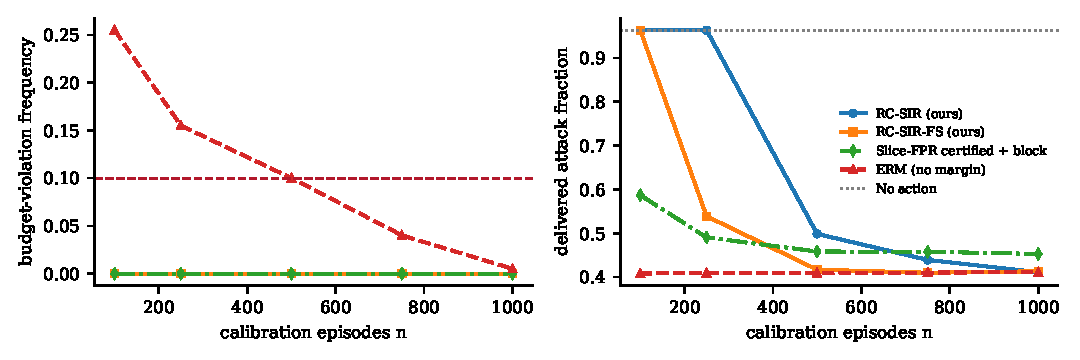
\includegraphics[width=0.95\textwidth]{figures/fig_ncal.pdf}\caption{Left: budget-violation frequency versus calibration size (dashed line: $\delta$). Right: delivered attack fraction versus calibration size.}\label{fig:ncal}\end{figure*}

\textbf{Load shift.} Calibrating on nominal-load episodes and testing on
high-load episodes produced no violations for RC-SIR-FS (0.000), because
collateral in this model is driven by acting on benign UEs, which load
changes little. Recalibrating on only 200 shifted episodes left too few
samples to certify any policy (fallback rate 1.00). We do not claim
robustness to shifts that change benign score distributions.

\textbf{Twin calibration.} Calibrating on a twin with 8\% optimistic
capacity, without correction, produced no violations (0.000). The
largest per-slice mean twin/real gap was 0.025 (eMBB). The rigorous
correction of Proposition 2 with \(m=300\) paired episodes subtracts a
Hoeffding term of about 0.14, larger than every budget, so the certified
set was always empty (fallback rate 1.00). A plug-in correction without
the concentration term retained most of the utility (0.489 delivered)
but is not covered by Proposition 2. A practical twin-transfer
certificate needs a tighter, policy-specific bound.

\textbf{Cost.}

\begin{itemize}
\tightlist
\item
  Selection and certification on 500 episodes took 4.6 ms (median).
\item
  Replay dominates: 7,064,900 policy--episode evaluations took 864 s on
  4 vCPUs, i.e.~0.122 ms each in this fluid model.
\item
  A packet-level twin or a testbed would be orders of magnitude slower
  per evaluation. This favours Slice-FPR whenever replay is expensive.
\end{itemize}

\begin{table*}[!t]
\centering
\caption{Measured harm ratio (Proposition 2) for single-slice policies over all 1500 pool episodes.}
\label{tab:harm_ratio}
\footnotesize
\resizebox{\linewidth}{!}{%
\begin{tabular}{lrlrrr}
\toprule
\textbf{Slice} & \textbf{Threshold} & \textbf{Action} & \textbf{Acted benign fraction} & \textbf{Collateral} & \textbf{Harm ratio rho} \\
\midrule
eMBB & 0.9 & RL & 0.2141 & 0.1373 & 0.641 \\
eMBB & 0.9 & block & 0.2141 & 0.1462 & 0.683 \\
eMBB & 0.95 & RL & 0.1336 & 0.0829 & 0.621 \\
eMBB & 0.95 & block & 0.1336 & 0.0868 & 0.650 \\
eMBB & 0.99 & RL & 0.0352 & 0.0190 & 0.541 \\
eMBB & 0.99 & block & 0.0352 & 0.0191 & 0.544 \\
eMBB & 0.995 & RL & 0.0132 & 0.0061 & 0.460 \\
eMBB & 0.995 & block & 0.0132 & 0.0061 & 0.460 \\
eMBB & 0.999 & RL & 0.0021 & 0.0009 & 0.400 \\
eMBB & 0.999 & block & 0.0021 & 0.0009 & 0.400 \\
URLLC & 0.9 & RL & 0.1009 & 0.0968 & 0.960 \\
URLLC & 0.9 & block & 0.1009 & 0.0982 & 0.974 \\
URLLC & 0.95 & RL & 0.0767 & 0.0731 & 0.954 \\
URLLC & 0.95 & block & 0.0767 & 0.0743 & 0.969 \\
URLLC & 0.99 & RL & 0.0026 & 0.0025 & 0.949 \\
URLLC & 0.99 & block & 0.0026 & 0.0025 & 0.949 \\
URLLC & 0.995 & RL & 0.0000 & 0.0000 & -- \\
URLLC & 0.995 & block & 0.0000 & 0.0000 & -- \\
URLLC & 0.999 & RL & 0.0000 & 0.0000 & -- \\
URLLC & 0.999 & block & 0.0000 & 0.0000 & -- \\
mMTC & 0.9 & RL & 0.0536 & 0.0069 & 0.129 \\
mMTC & 0.9 & block & 0.0536 & 0.0527 & 0.982 \\
mMTC & 0.95 & RL & 0.0031 & 0.0003 & 0.107 \\
mMTC & 0.95 & block & 0.0031 & 0.0031 & 0.987 \\
mMTC & 0.99 & RL & 0.0000 & 0.0000 & -- \\
mMTC & 0.99 & block & 0.0000 & 0.0000 & -- \\
mMTC & 0.995 & RL & 0.0000 & 0.0000 & -- \\
mMTC & 0.995 & block & 0.0000 & 0.0000 & -- \\
mMTC & 0.999 & RL & 0.0000 & 0.0000 & -- \\
mMTC & 0.999 & block & 0.0000 & 0.0000 & -- \\
\bottomrule
\end{tabular}
}
\end{table*}

\hypertarget{sec:discussion}{%
\section{Discussion}\label{sec:discussion}}

The answer to the research question is conditional. Certifying
action-induced collateral directly admitted more mitigation than
certifying false-positive rates only when three conditions held:

\begin{enumerate}
\def\labelenumi{\arabic{enumi}.}
\tightlist
\item
  the harm ratio of the slice that limits the policy was well below one;
\item
  the threshold grid had points in the resulting band;
\item
  there were enough calibration episodes for a powerful testing
  procedure (fixed-sequence ordering rather than Bonferroni).
\end{enumerate}

When any of these failed, per-slice FPR certification was as good or
better, and much cheaper, because it needs only benign detector scores
rather than counterfactual replays.

For operators this suggests a practical order of work:

\begin{enumerate}
\def\labelenumi{\arabic{enumi}.}
\tightlist
\item
  Certify per-slice FPR first. Under a monotone scheduler (Lemma 1) it
  already bounds collateral.
\item
  Estimate harm ratios per slice and action.
\item
  Invest in replay-based certification only where those ratios are
  small.
\end{enumerate}

\hypertarget{sec:limits}{%
\section{Limitations and Threats to Validity}\label{sec:limits}}

\textbf{Simulation only.} All results come from a fluid model of a
three-slice egress link with synthetic traffic, not from a 5G core, a
RAN or real traces. The checkpoint that preceded this study found no
accessible testbed. 5G-NIDD \cite{siriwardhana2025nidd} could not be
retrieved in the execution environment, and it carries no slice labels
or SLA outcomes, so it could not supply \(L^c_s\). The guarantees are
properties of the procedure under A1--A3 and do not depend on the
simulator; the \emph{utility} comparisons do.

\textbf{Assumption A3.} Monotonicity was verified for our scheduler, not
for real UPF implementations. Congestion-controlled transports, active
queue management and adaptive application behaviour can violate it. If
A3 fails, Lemma 1 and Corollary 1 fail, and per-slice FPR certification
no longer bounds collateral. Direct certification (Proposition 1) does
not need A3.

\textbf{Design iterations, disclosed.}

\begin{enumerate}
\def\labelenumi{\arabic{enumi}.}
\tightlist
\item
  \emph{First traffic model.} It used a single regime and gave a
  detector with AUC 0.99999, under which every method trivially met its
  budgets. We replaced it with the train/deploy regime model before
  analysing method results, and archived it.
\item
  \emph{Objective.} The first full analysis used the benign-violation
  index \(J\) as the selection objective, contrary to the pre-specified
  formulation (minimise \(R^a\)). Under \(J\) the constraints were never
  active and no method violated its budgets. We corrected the objective;
  the \(J\)-objective results are archived.
\item
  \emph{Recommended variant.} Both certification variants were specified
  before results. Recommending the fixed-sequence variant is a post-hoc
  choice that the results motivated.
\end{enumerate}

The full record is in \texttt{DESIGN\_LOG.md} and
\texttt{research\_decisions.md}.

\textbf{Statistics.}

\begin{itemize}
\tightlist
\item
  The 200 splits reuse one pool of 1500 episodes, so split-level
  summaries describe variability over calibration draws, not independent
  replications. We therefore report quantiles and win fractions rather
  than p-values for method differences.
\item
  A violation frequency of zero over 200 splits is consistent with the
  target \(\delta=0.1\), but it does not show that the bound is tight.
  The budgets were rarely binding for certified methods.
\end{itemize}

\textbf{Episodes.} Actions are fixed for the whole action window.
Episodes are i.i.d. by construction, whereas real traffic has temporal
dependence that A1 ignores.

\textbf{Baselines not reproduced.} Model-based intrusion-response
policies \cite{hammar2022optimalstopping, hammar2024dynamic} require an
attacker model and simulator interface that we did not reimplement
faithfully. They optimise a different criterion and provide no
collateral certificate, so they would answer a different question.

\hypertarget{sec:conclusion}{%
\section{Conclusion}\label{sec:conclusion}}

We asked whether certifying the per-slice SLA collateral of mitigation
actions buys more attack mitigation than certifying per-slice
false-positive rates. Under a monotone user-plane scheduler,
false-positive certification already bounds collateral. Direct
certification can only exploit the harm ratio, at the price of
counterfactual replay and a larger hypothesis space.

In our simulation study both certified approaches always met their
budgets, while uncalibrated selection did not. Direct certification with
fixed-sequence testing reduced delivered attack traffic relative to
per-slice FPR certification in most calibration draws at nominal budgets
and moderate calibration sizes. It lost that advantage with small
calibration sets, at other budget levels, and with Bonferroni control.

Validating A3 on a real UPF, obtaining slice-labelled traces with SLA
outcomes, and tightening twin-transfer bounds are the steps needed
before these findings can inform deployment.
